\chapter{Aprendizaje profundo. Fundamentos}\label{ch:quinto-capitulo}

\section{Descripción de un modelo formal de Aprendizaje Automático}\label{sec:4.1}

El Aprendizaje Automático comprende una serie de prácticas y algoritmos que comparten como objetivo común la tarea de aprender información a partir de unos datos de entrada.  La descripción formal para un modelo de Aprendizaje Automático suele tener los siguientes elementos: 

\begin{itemize}
\item Dominio del problema: se trata de un conjunto $X$ que contendrá todos los objetos que tenemos a nuestra disposición para realizar la tarea de aprendizaje. 
%\item Conjunto de etiquetas: 
\item Conjunto de entrenamiento: Un conjunto finito de datos $S\subset X$, donde $X$ es el espacio del dominio del problema. En caso de tratarse de un problema de aprendizaje supervisado, $S=\{(x_{1},y_{1}),\ldots,(x_{n},y_{n}\}\}\subset X\times Y$, donde $X$ e $Y$ son respectivamente el espacio del dominio del problema y su conjunto de etiquetas asociado. 
\item Una hipótesis de aprendizaje que el algoritmo $A$ construye tras haber recibido el conjunto de entrenamiento $S$. La denotaremos por $A(S)$.
\item Un predictor $h:X\rightarrow Y$ devuelto por el algoritmo tras la tarea de aprendizaje que describe la hipótesis $A(S)$.
\item Una medida de bondad de la predicción realizada por el algoritmo. Esta medida tiene el nombre de función de coste y está asociada a la probabilidad de que, dado un elemento arbitrario $x\in X$, el algoritmo comenta un error en la predicción.
\end{itemize}

Este modelo tan general se ha concretado en varios modelos de aprendizaje. En este trabajo nos centraremos en describir las principales características del Aprendizaje Profundo, cuyo objeto de interés principal son las redes neuronales.


\section{Redes Neuronales Artificiales}

 Una Red Neuronal Artificial (RNA) es un modelo de Aprendizaje Automático basado en la idea de que muchas unidades de cómputo pequeñas pueden unirse y comunicarse para construir modelos complejos. Para ello, imitan estructura y el comportamineto de las neuronas biológicas. Esta idea surge en 1943 ~\cite{mcculloch1943logical} de la mano del neurofisiólogo Warren McCulloch y el matemático Walter Pitts, quienes diseñaron el primer modelo de neurona artificial. En las décadas posteriores a su descubrimiento se fueron explorando nuevas arquitecturas, como el perceptrón multicapa. Sin embargo, en este momento su capacidad de aprendizaje era muy limitada. En los años 80, la popularización del algoritmo de retropropagación dio nuevas esperanzas a las redes neuronales, pero sus altos requerimientos computacionales, como el uso de GPU, hicieron que el interés general fuese a otras técnicas de aprendizaje automático que habían surgido en la época, como SVM. Sin embargo, en los últimos años las redes neuronales profundas han demostrado ser capaces de abordar tareas complicadas que otras técnicas no son capaces de abordar, y se han convertido en el objeto de muchas tareas de investigación.
 
\subsection{Tipos de redes neuronales}
Una de las grandes ventajas de las redes neuronales es su flexibilidad para aprender en tareas con objetivos muy dispares. Es por esto que a partir de los años 90, aparecen distintas arquitecturas que facilitan tareas de aprendizaje con distintos objetivos. Entre ellas destacan: 

\begin{itemize}
    \item Redes neuronales prealimentadas (MLP): Están compuestas por una capa de entrada, una capa de salida y, entre ellas, una o varias capas llamadas capas ocultas. Cada neurona está conectada a todas las neuronas de su capa siguiente y, análogamente, cada neurona de la capa de salida está contectada a todas las neuronas de la capa anterior. Son utilizadas para tareas de clasificación, regresión y aproximación de funciones. 
    \item Redes neuronales convolucionales (CNN): Compuestas por capas de convolución en las que se aplican filtros para extraer características locales de los datos que la capa siguiente toma como entrada. Se utilizan principalmente para reconocimiento de imágenes.  
    \item Redes neuronales recurrentes (RNN): Las conexiones entre neuronas forman ciclos, lo que les permite mantener una memoria interna de las secuencias de datos que entran a la red. Pueden utilizarse para procesamiento del lenguaje natural y para predicción de secuencias. 
\end{itemize}

\section{Redes Neuronales Prealimentadas} 
 En~\cite{shalev-shwartz2014understanding} se describe una red neuronal prealimentada como un grafo dirigido acíclico $G=(V,E)$  organizado por capas, $V=\{V_{0},V_{1},\ldots,V_{n}\}$, con una función de pesos $w: E\rightarrow \mathds{R}$ asociada.  Como puede verse en la \autoref{fig:img01}, los vértices representan neuronas artificiales (unidades de cómputo simple) y las aristas representan las conexiones entre ellas. Supongamos que la capa $i$ tiene $n$ neuronas. Entonces, denotaremos $V_{i} = \{v_{i,1},\dots v_{i,n}\}$ a las neuronas en esa capa. Si tenemos una red neuronal con  $T+1$ capas, $V_{0},\dots,V_{T}$, llamamos a $V_{0}$ capa de entrada, a $V_{T}$ capa de salida y a las capas $\{V_{1},\dots , V_{T-1} \}$ capas ocultas. Una red neuronal profunda es aquella que tiene un número considerable de capas ocultas. 

 Aunque hayamos considerado todas las neuronas como unidades de cómputo simple, es importante remarcar que en la capa de entrada $V_{0}$ no se realiza ningún cálculo: únicamente se procesan los datos de entrada. Esta capa tiene tantas neuronas como dimensiones tenga un dato de entrada además de una neurona extra, que recibe una entrada constante y que sirve como término de sesgo. 
 
Para el resto de capas $V_{1},\dots ,V_{T}$, una neurona sí conforma una unidad de cómputo. Así, en cada neurona $v_{i,j}$ de la capa $i$, con $i=1,\dots,T$, se realiza una suma ponderada de las entradas que le llegan de la capa anterior, esto es, se realiza la operación $z = w^{T}x+b$ donde el vector $w$ viene dado por la función de pesos asociada a la red neuronal, $x$ representa las salida de las neuronas de la capa $i-1$ conectadas a $v_{i,j}$y $b$ es, de nuevo, un término de sesgo. A esta suma ponderada se aplica una función real, a la que llamaremos función de activación. \\ 
 \begin{figure}[ht]
    \centering
    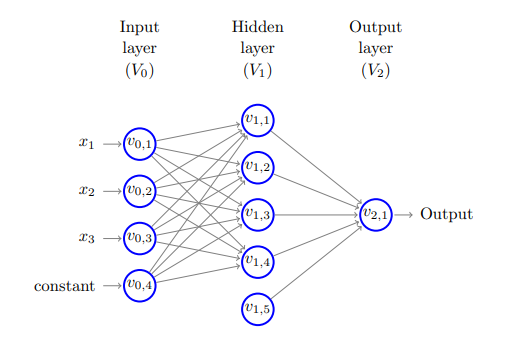
\includegraphics[width=0.5\textwidth]{img/img01.png}
    \caption{Arquitectura de Red Neuronal presentada en  ~\cite{shalev-shwartz2014understanding}.}
    \label{fig:img01}
\end{figure}

 Las redes neuronales profundas han supuesto un antes y un después en el Aprendizaje Automático ya que su arquitectura les permite aprender patrones complejos y abstractos: las capas inferiores (las más próximas a la capa de entrada) aprenden relaciones simples entre los datos, las capas siguientes, partiendo de esas relaciones simples, consiguen encontrar relaciones más abstractas sobre ellas, dando lugar a un aprendizaje más complejo y general conforme vamos llegando a las capas superiores (las capas cercanas a la de salida). \\


Con esta estructura, una red neuronal prealimentada define una aplicación $f(x,w)$ y aprende los valores de $w$ que llevan a la mejor aproximación de $y$. En una red prealimentada, la información únicamente fluye hacia delante antes de ser evaluada, en contraposición a lo que ocurre con las redes neuronales recurrentes mencionadas en el apartado anterior. 

\subsection{Funciones de Activación}
Una de las cuestiones más importantes a la hora de definir una red neuronal es la elección de una función de activación adecuada para cada capa de neuronas. De hecho, la elección de funciones de activación demasiado simples fue, históricamente, una de las principales razones por las que las redes neuronales fueron consideradas poco capaces en sus inicios. La correcta elección de funciones de activación depende principalmente de tres factores: 


\begin{itemize}
    \item Objetivo de la tarea de aprendizaje: en la capa de salida, es posible que necesitemos funciones de activación que describan una distribución de probabilidad (clasificación binaria), probabilidad conjunta (clasificación multiclase) o que respondan a otro tipo de comportamiento, lineal o no (regresión).
    \item Complejidad de la tarea de aprendizaje: para tareas complejas, algunas funciones de activación pueden no ser suficientes.
    \item Compatibilidad de la función de activación con el algoritmo de entrenamiento de la red neuronal: los algoritmos que definen y  optimizan el entrenamiento de una red neuronal, además de los que regularizan el modelo final, pueden comportarse mejor si las funciones de activación cumplen unos requisitos de derivabilidad y preservación de la varianza. Entraremos en estos detalles más adelante. 
\end{itemize}
En el contexto del Aprendizaje Profundo, algunas de las funciones de activación más utilizadas son: 
\begin{itemize}
    \item Sigmoidal: Es una de las funciones de activación más utilizadas. Sin embargo, se ha demostrado que no preserva bien la varianza de los datos de entrada, lo que puede dar problemas de gradientes inestables durante el entrenamiento.
    \begin{equation}
        \sigma (z) = \frac{1}{1+e^{-(z)}}
    \end{equation}
    \begin{figure}[htbp]
        \centering
        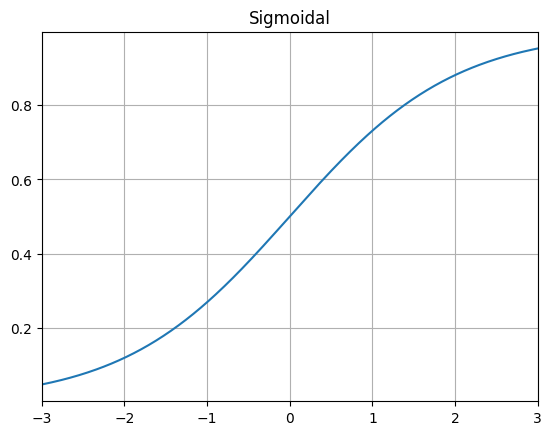
\includegraphics[width=0.4\textwidth]{img/img21.png}
        \caption{Función de activación sigmoidal.}
        \label{fig:img21}
    \end{figure}
    
    \item Tangente hiperbólica: Como se puede ver en la \autoref{fig:img22}, tiene una media cercana a $0$, lo que ayuda a preservar la varianza más que la función sigmoidal.
    \begin{equation}
        tanh(x) = \frac{e^{x}-e^{-x}}{e^{x}+e^{-x}}
    \end{equation}
    \begin{figure}[htbp]
        \centering
        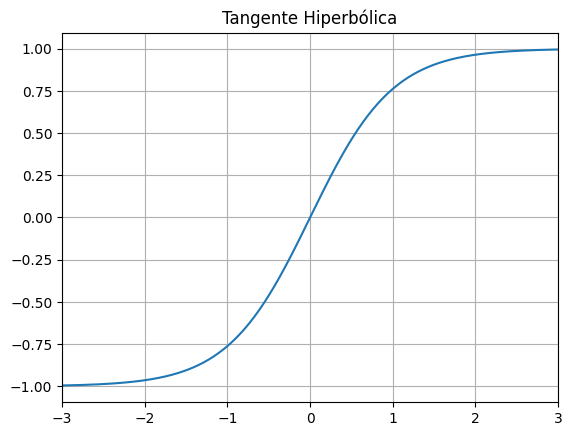
\includegraphics[width=0.4\textwidth]{img/img22.png}
        \caption{Función de activación tangente hiperbólica.}
        \label{fig:img22}
    \end{figure}
    
    \item Lineal rectificada (ReLU): Entre sus ventajas destacan su simplicidad de cómputo. Suele funcionar muy bien en redes neuronales profundas.
    \begin{equation}
        ReLU(x) = max(0,x)
    \end{equation}
    \begin{figure}[htbp]
        \centering
        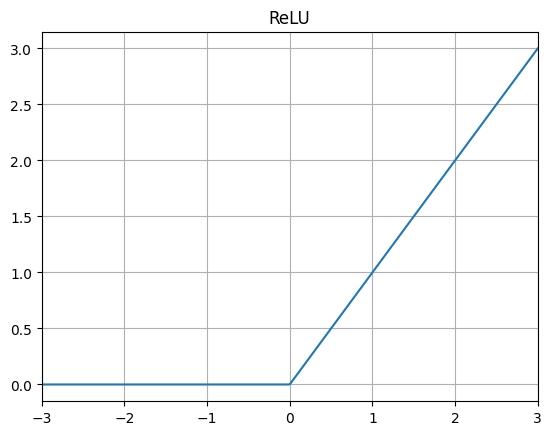
\includegraphics[width=0.4\textwidth]{img/img23.png}
        \caption{Función de activación ReLU.}
        \label{fig:img23}
    \end{figure}
    
    \item Leaky ReLU: Conocida como ReLU con fugas, garantiza un gradiente positivo para todo $z<0$ mediante el hiperparámetro de grado de fuga $\alpha$.  Esto garantiza que para salidas $z<0$ las neuronas nunca mueran. 
    \begin{figure}[htbp]
        \centering
        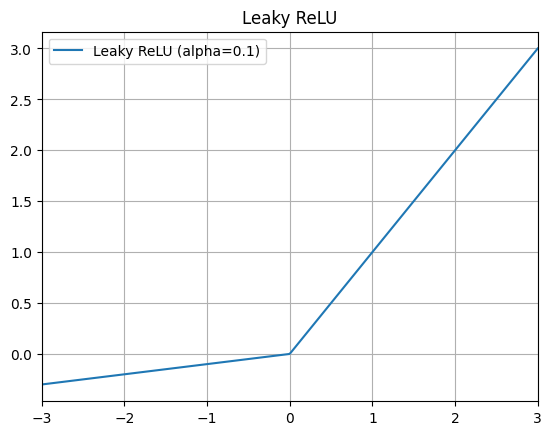
\includegraphics[width=0.4\textwidth]{img/img24.png}
        \caption{Función de activación Leaky ReLU.}
        \label{fig:img24}
    \end{figure}
    \item ELU y SELU:  Toma valores negativos, lo que permite que sus valores medios de salida sean más cercanos a $0$. Además es suave para $\alpha = 1$, lo que ayuda a acelerar el descenso de gradiente para valores ceranos a $0$. SELU~\cite{klambauer2017self} es una versión escalada de ELU con $\alpha=1.67$ que ayuda a la autonormalización de redes neuronales densas. 
    \begin{equation}
        ELU_{\alpha}(z) = 
        \begin{cases}
             \text{ } \alpha (e^{z}-1) \quad & si \text{ } z<0 \\
             \text{ } z \quad & si  \text{ } z \geq 0
        \end{cases}
    \end{equation}
    \begin{figure}[htbp]
        \centering
        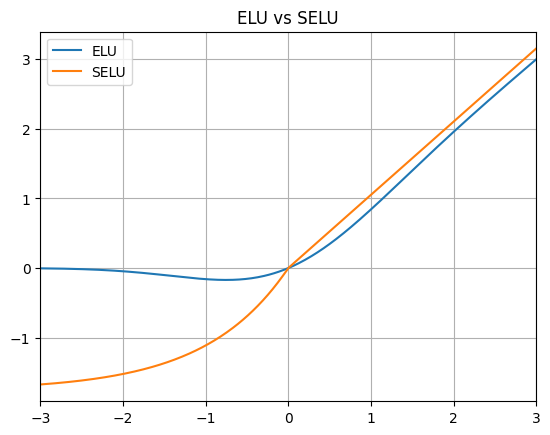
\includegraphics[width=0.4\textwidth]{img/img26.png}
        \caption{Funciones de activación ELU y SELU.}
        \label{fig:img26}
    \end{figure}
    \item GELU: Presentada en~\cite{hendrycks2016gaussian}, es parecida a las funciones ReLU y ELU pero, a diferencia de ellas, no es convexa ni monótona. Su buen funcionamiento se atribuye a tener una curvatura distinta en cada punto.
    \begin{figure}[htbp]
        \centering
        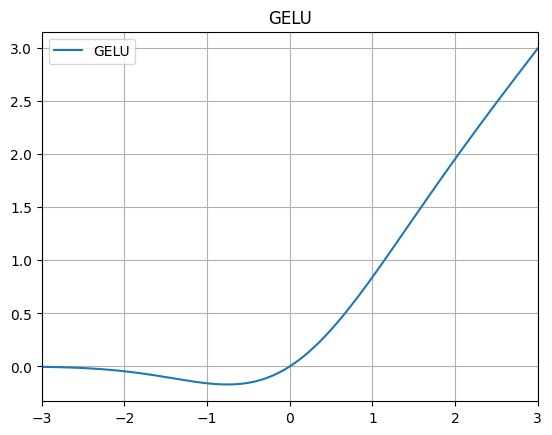
\includegraphics[width=0.4\textwidth]{img/img25.png}
        \caption{Función de activación GELU.}
        \label{fig:img25}
    \end{figure}
\end{itemize}

\subsection{Función de coste}

Aunque es posible orientar el aprendizaje de una red neuronal hacia varios propósitos, en este trabajo vamos a centrarnos en el uso de redes neuronales para aprender funciones, funcionales y operadores. Para esta tarea, los elementos formales descritos en la \autoref{sec:4.1} se asemejan a los de un problema de regresión.

El objetivo del aprendizaje será, por tanto, encontrar el conjunto de parámetros que minimiza una métrica de error (generalmente, el error cuadrático medio) con respecto a una función, funcional u operador. Recordemos que los parámetros asociados a una red neuronal son el conjunto de pesos $\theta = \{ w(E) \}$. La función de coste asociada a $\theta$, $J(\theta)$, estará relacionada con la métrica de error.


\subsection{Entrenamiento}

\subsubsection{Optimización}\label{sec:4.3.3.1}
Como buscamos minimizar $J(\theta)$ en función de $\theta$, no es de extrañar que el algoritmo de descenso de gradiente forme parte del proceso de entrenamiento en redes neuronales prealimentadas. Este algoritmo de optimización genérico es capaz de encontrar soluciones óptimas a una amplia gama de problemas. La idea general del descenso de gradiente es ajustar 
los parámetros de forma iterativa para minimizar la función de 
coste. Para ello, cada vez que un lote de información se propaga hasta la capa de salida, se realiza un paso de descenso de gradiente. Esto es, sobre el conjunto de pesos $\theta$, se computa 

\begin{equation}
    \theta^{siguiente} = \theta - \eta\nabla_{\theta}J(\theta)
\end{equation}

donde $\eta$ es la tasa de aprendizaje, parámetro que indica cómo de brusco será el paso de descenso de gradiente. 


En el contexto de entrenamiento de redes neuronales para la predicción de funciones complejas, el descenso de gradiente tiene varios problemas como su elevado coste computacional, su sensibilidad a cambios bruscos en la pendiente de $J(\theta)$ y su riesgo de caer en mínimos locales sin alcanzar el mínimo global del problema. Esto hace que para este tipo de problemas se escojan versiones alternativas del algoritmo que favorecen la tarea de aprendizaje. 


\subsubsection{Propagación hacia atrás}

Aunque obtener la expresión analítica de un paso de descenso de gradiente es, como hemos visto, sencillo, evaluar numéricamente esa expresión puede llegar a ser muy costoso. En 1970, el investigador Seppo Linnainmaa introdujo en su tesis de máster~\cite{linnainmaa1970representation} una técnica para calcular los gradientes de forma automática y eficiente mediante la regla de la cadena. Este algoritmo se denomina ahora diferenciación automática en modo inverso. El algoritmo de propagación hacia atrás (back propagation), que combina esta técnica con el descenso de gradiente, mitiga los problemas de coste de este último y es el algoritmo estándar utilizado para ajustar $\theta$ tras el cálculo del error (es decir, en el paso hacia atrás). 


\subsubsection{Tasa de Aprendizaje}

Uno de los grandes retos del correcto entrenamiento de una red neuronal es encontrar el valor adecuado para la tasa de aprendizaje. Como vemos en la \autoref{fig:img17}, cuando usamos una tasa demasiado grande, los pasos de descenso de gradiente escapan el mínimo local, haciendo que el algoritmo diverja.

 \begin{figure}[htbp]
    \centering
    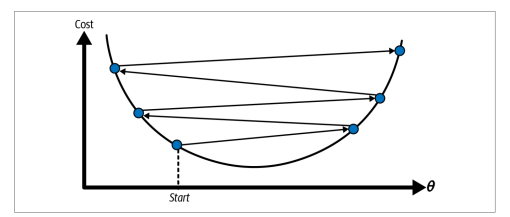
\includegraphics[width=0.5\textwidth]{img/img17.png}
    \caption{Pasos de descenso de gradiente para una tasa de aprendizaje demasiado grande. Imagen extraída de~\cite{Buric2020}.}
    \label{fig:img17}
\end{figure}

Por otro lado, si la tasa de aprendizaje es demasiado pequeña, como en la \autoref{fig:img18}, necesitaremos demasiadas etapas de entrenamiento para llegar al mínimo local. Es posible que el entrenamiento se detenga antes de alcanzar ese mínimo. 

 \begin{figure}[htbp]
    \centering
    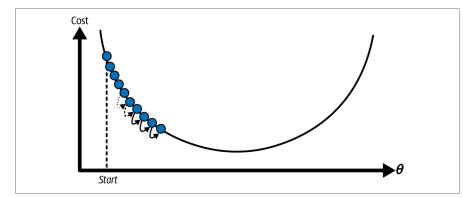
\includegraphics[width=0.5\textwidth]{img/img18.png}
    \caption{Pasos de descenso de gradiente para una tasa de aprendizaje demasiado pequeña. Imagen extraída de~\cite{Buric2020}.}
    \label{fig:img18}
\end{figure}

El valor óptimo para la tasa de aprendizaje es aquel que minimiza el número de pasos de descenso de gradiente a realizar antes de alcanzar el mínimo local de $J(\theta)$. Para este valor, los pasos de descenso de gradiente se comportan como en la \autoref{fig:img19}.

 \begin{figure}[htbp]
    \centering
    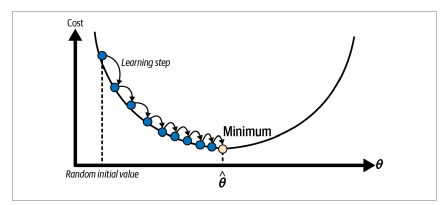
\includegraphics[width=0.5\textwidth]{img/img19.png}
    \caption{Pasos de descenso de gradiente para una buena tasa de aprendizaje. Imagen extraída de~\cite{Buric2020}.}
    \label{fig:img19}
\end{figure}

En la \autoref{sec:4.3.3.1} comentábamos que el algoritmo de descenso de gradiente es sensible a cambios bruscos de pendiente. Esto se debe a que no todas las funciones de coste son convexas como en las gráficas anteriores. En muchas ocasiones la función de coste presenta tramos con pendientes muy distintas, lo que hace que, como se puede observar en la \autoref{fig:img20}, una tasa de aprendizaje que funcione bien en un tramo, pueda no ser adecuada en otro.  \\
 \begin{figure}[htbp]
    \centering
    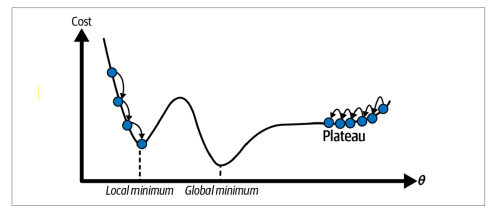
\includegraphics[width=0.5\textwidth]{img/img20.png}
    \caption{Tasa de aprendizaje constante para una función de coste con cambios bruscos en la pendiente. Imagen extraída de~\cite{Buric2020}. }
    \label{fig:img20}
\end{figure}

Es por esto que, especialmente en tareas complejas, se opta por optimizadores que adaptan la tasa de aprendizaje a la etapa de entrenamiento o por programar el ritmo de aprendizaje. Entre las programaciones más utilizadas destacan: 

\begin{itemize}
    \item Power Scheduling: Modifica la tasa de aprendizaje en función del número de iteración $t$. El comportamiento viene descrito por: $\eta (t) = \frac{\eta_0}{(1+\frac{t}{s})^c} $, donde $\eta_0$ es la tasa de aprendizaje inicial, $s$ el paso de decay y $c$ suele fijarse a $1$. Esta técnica requiere afinar los hiperparámetros mencionados.
    \item Performance Scheduling: Reduce la tasa de aprendizaje en un factor $\lambda$ cuando el error de validación deja de decaer. 
    
    \item Programación exponencial: Reduce la tasa de aprendizaje en un factor de $10$ cada $s$ pasos. Este comportamiento viene dado por $\eta(t)=\eta_0 0.1^{\frac{t}{s}}$. 
    \item Programación constante a trozos: Consiste en asociar valores de tasa de aprendizaje a un número de épocas determinado. Esta aproximación es la más sensible a ajuste de parámetros. 
\end{itemize}

\subsubsection{Optimizadores más rápidos}

Además de una buena elección de funciones de activación y de un valor adecuado para la tasa de aprendizaje, otro aspecto clave para la eficiencia en el aprendizaje viene dado por el algoritmo de optimización escogido para la función de coste. En la \autoref{sec:4.3.3.1} presentábamos cómo se usa el algoritmo de descenso de gradiente en redes neuronales prealimentadas. Como pudimos ver, este algoritmo realiza pasos constantes y actualiza el gradiente de la función de coste atendiendo únicamente al gradiente local, esto es, sin considerar los valores de gradiente anteriores. Esto se traduce en que no es capaz de coger velocidad cuando nos encontramos cerca del mínimo, lo que ralentiza el proceso de aprendizaje. 

La primera respuesta a esta problemática surgió en 1964 de la mano de Boris Polyak, quien propuso la optimización basa en el momentum, la cual introduciremos a continuación. En esta sección introduciremos algunas variantes del descenso de gradiente inspiradas esta idea. 

\begin{itemize}
    \item Momentum: tiene en cuenta el gradiente local, pero lo utiliza como aceleración, no como velocidad. Para ello, el vector de gradientes se actualiza de forma: 
    \begin{enumerate}
        \item $m \leftarrow \beta m - \eta \nabla_\theta J(\theta) $
        \item $\theta \leftarrow \theta + m$ 
    \end{enumerate}
    donde $m$ es el vector de momentos y el parámetro $\beta$, denominado \textit{momentum}, simula una fricción que evita que $m$ crezca demasiado. Suele escogerse $\beta = 0.9$. 

    \item Gradiente acelerado de Nesterov: Es una variante de Momentum introducida por Yurii Nesterov en 1983. Propone evaluar la función de coste en $\theta+ \beta m$ en vez de en $\theta$. Este cambio se debe a que, en general, el vector $m$ toma direcciones que apuntan más al óptimo que $\theta$. Este empuje en la dirección correcta se implementa como sigue:
    \begin{enumerate}
        \item $m \leftarrow \beta m - \eta \nabla_\theta J(\theta + \beta m) $
        \item $\theta \leftarrow \theta + m$. 
    \end{enumerate}

    \item AdaGrad: Corrige la tendencia natural del descenso de gradiente por la pendiente más pronunciada, que no tiene por qué apuntar al óptimo global. Esto se logra escalando el vector de gradiente. De este modo, el algoritmo hace decaer la tasa de aprendizaje más rápido para direcciones empinadas y más despacio en direcciones de gradiente más suave. Este algoritmo funciona bien para problemas sencillos, pero funciona mal en modelos complejos de aprendizaje profundo, donde la tasa de aprendizaje puede reducirse tanto que no se llegue a alcanzar el óptimo global. Para ello, en cada etapa se calcula:
    \begin{enumerate}
        \item $s \leftarrow s +  \nabla_\theta J(\theta)\otimes \nabla_\theta J(\theta) $
        \item $\theta \leftarrow \theta -\eta \nabla_\theta J(\theta)\oslash\sqrt{s+\varepsilon}$
    \end{enumerate}
    donde $\otimes$ representa el producto elemento a elemento, por lo que $s$ acumula el cuadrado de los gradientes. 
    

    \item RMSProp: Soluciona el riesgo que corre Adagrad de acabar el entrenamiento demasiado pronto acumulando los gradientes de las iteraciones más recientes. Así,  obtenemos:
    \begin{enumerate}
        \item $s \leftarrow \rho s + (1-\rho) \nabla_\theta J(\theta)\otimes \nabla_\theta J(\theta) $
        \item $\theta \leftarrow \theta -\eta \nabla_\theta J(\theta)\oslash\sqrt{s+\varepsilon}$
    \end{enumerate}
    donde el parámetro $\rho$, que suele fijarse en $0.9$, representa el decaimiento exponencial que introduce el algoritmo para mitigar el problema. 

    \item Estimación adaptativa por momentos (Adam): Combina las idea de Momentum y RMSProp. Para ello, se realizan los siguientes pasos: 
    \begin{enumerate}
        \item $m \leftarrow \beta_1 m - (1-\beta_1) \nabla_\theta J(\theta) $
        \item $s \leftarrow \beta_2 s + (1-\beta_2) \nabla_\theta J(\theta)\otimes \nabla_\theta J(\theta) $
        \item $\hat{m} \leftarrow \frac{m}{1-\beta_1^t}$
            \item $\hat{s} \leftarrow \frac{s}{1-\beta_2^t}$
        \item $\theta \leftarrow \theta + \eta \hat{m} \oslash \sqrt{\hat{s}+\varepsilon}$.
    \end{enumerate}
    Es un algoritmo ampliamente utilizado. Al contar con una tasa de aprendizaje adaptativa, requiere menos ajustes y es cómodo de utilizar.  

    \item Nesterov-accelerated Adaptive Moment (Nadam): Es una variante de Adam que aplica la idea de aceleración de Nesterov. Suele converger más rápido que Adam. 

\end{itemize}